\documentclass[11pt]{article}      
\usepackage[a4paper,                
top=1in,                         
bottom=1in,                       
left=1in,                         
right=1in]{geometry} 

\setlength\parindent{0pt}
                                    
\usepackage[english]{babel}
\usepackage{amsfonts} 
\usepackage{amsmath}
\usepackage{amsthm}
\usepackage{amssymb}
\usepackage{mathtools} 
\usepackage{graphicx} 
\usepackage{xcolor}
\usepackage{bbm}
\usepackage{float}
\usepackage{verbatim}
\usepackage{tikz}
\usepackage{subcaption}

\usepackage[colorlinks=true, linkcolor=blue]{hyperref}
\usepackage{hyperref}

\usepackage{tikz}
\usetikzlibrary{shapes.geometric, positioning}
\usetikzlibrary{arrows.meta, positioning, calc}

\thinmuskip=4mu
\medmuskip=6mu
\thickmuskip=8mu

\begin{document}
\begin{figure}[t!]
\centering
\includegraphics[width=60mm]{Latex/logoEPFL.png}
\end{figure}

\begin{center}
{\Large \textbf{Numerical Flow Simulation  - Project 1}}\\
\vspace{2mm}
{\large Yanpeng Zhang, Stefano Bernasconi, Pietro Fumagalli, Francesco Derme}\\
{\large 394469, 414363, 414991, 394806}
\end{center}

\vspace{2.5pt}
\paragraph{Setup.}
Consider a fluid flowing through a plane channel between horizontal walls located in $y = 0$ and $y = H$ as shown in Figure \ref{channel_domain}. The temperature field $T(x, y)$ is the solution of the steady heat equation, $\nabla\cdot(\rho\,u\,T)=\nabla\cdot(\Gamma\,\nabla T)$. Here, the density $\rho$, the velocity field $u$=$[u_x , u_y]^T$ and the thermal properties are known ($\Gamma = k/c_p$ is the ratio of thermal conductivity $k$ to specific heat capacity $c_p$). Assume that $T$ is a passive scalar, i.e. the fluid properties and the velocity field are independent of temperature. The two-dimensional numerical domain is a simple rectangle such that $0 \leq x\leq L$ and $0 \leq y \leq H$. Also, consider a structured mesh with $n_x$ cells in the $x$ direction and $n_y$ cells in the $y$ direction, then $\Delta x = L/(n_x-1)$, $\Delta y = H/(n_y-1)$. Here, the denominator is $n_x - 1$ instead of $n_x$ because the boundary control volumes, as will be explained later, are cut in half so that their nodes sit exactly on the inlet, outlet or the walls. Indices $i, j$ range from 1 to $n_y, n_x$ respectively. By convention, the origin $(x,y)=(0,0)$ corresponds to the upper-left corner of the domain and thus to the center of the upper-left control-volume which is indexed by $(i,j)=(1,1)$, while $(i,j)=(n_y,n_x)$ are the indexes of the center of the bottom-right CV.
\begin{figure}[h!]
    \centering
    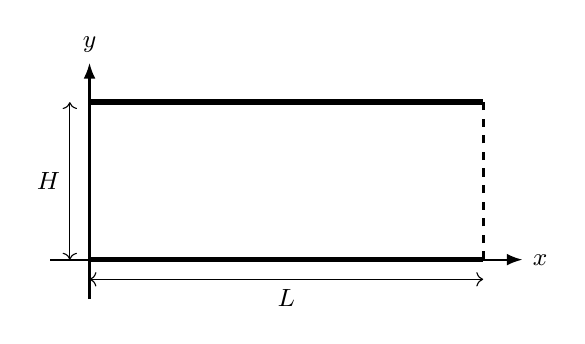
\begin{tikzpicture}[
        scale=0.5,
        font=\small
    ]
        \coordinate (origin) at (0,0);
        \coordinate (L_end) at (10,0);
        \coordinate (H_end) at (0,4);  
        \coordinate (LH_end) at (10,4);

        \draw[line width=2pt, fill=gray!10] (origin) -- (L_end);
        \draw[line width=2pt, fill=gray!10] (H_end) -- (LH_end);
        
        %\draw[dashed, line width=1pt] (origin) -- (H_end);
        \draw[dashed, line width=1pt] (L_end) -- (LH_end);

        \draw[->, thick, -{Latex[length=2mm]}] (-1,0) -- (11, 0) node[right] {$x$};
        \draw[->, thick, -{Latex[length=2mm]}] (0,-1) -- (0, 5) node[above] {$y$};
        %\node[below left=1mm and 1mm] at (origin) {$(0,0)$};

        \draw[<->] (0, -0.5) -- (10, -0.5);
        \node[below] at (5, -0.5) {$L$};
        \draw[<->] (-0.5, 0) -- (-0.5, 4);
        \node[left] at (-0.5, 2) {$H$};

    \end{tikzpicture}    
    \caption{Schematic of the 2D plane channel flow domain.}
    \label{channel_domain}
\end{figure}


\bigskip

\textbf{1. Fully developed laminar velocity.}
Consider the Navier-Stokes equations for the steady, incompressible case. Mathematically, to be \textit{fully developed} means $\partial_x u_x=0 \land \partial_x u_y=0$. Then, the spanwise momentum equation gives $\partial_y p=0$ and the continuity equation is $\partial_y u_y = \partial_x u_x = 0 \implies u_y$ is constant, so $u_y \equiv 0$ since $u_y(0) = u_y(H) = 0$ by the no-slip condition. The streamwise momentum equation instead reduces to
\[
0=-\frac{\mathrm{d}p}{\mathrm{d}x}+\mu\,\frac{\mathrm{d}^2 u_x}{\mathrm{d}y^2},
\]
subject to $u_x(0)=u_x(H)=0$. Integrating twice and applying boundary conditions gives
\[
u_x(y)=-\frac{1}{2\mu}\frac{\mathrm{d}p}{\mathrm{d}x}\,y(H-y),
\]
by symmetry the maximum lies at $y=H/2$
\[
u_{\max}=-\frac{1}{8\mu}\frac{\mathrm{d}p}{\mathrm{d}x}H^2.
\]
The mean velocity can be computed as
\[
u_{\mathrm{mean}}=\frac{1}{H}\int_0^{H}u_x(y)\,\mathrm{d}y=-\frac{1}{12\mu}\frac{\mathrm{d}p}{\mathrm{d}x}H^2,
\]
leading to to $u_{\max}=\tfrac{3}{2}\,u_{\mathrm{mean}}$. Finally,
\begin{align*}
u_x(y) &= u_{\max}\!\left[1 - \Bigl(2\frac{y}{H}-1\Bigr)^2\right] = 4u_{\max}\,\frac{y}{H}\!\left(1 - \frac{y}{H}\right) \\
u_x(y) &= 6u_{\mathrm{mean}}\,\frac{y}{H}\!\left(1 - \frac{y}{H}\right)\\
u_y(y) &= 0
\end{align*}

\bigskip

\textbf{2. Integral form on one CV.}
Consider the steady heat equation $\nabla\cdot(\rho\,u\,T)=\nabla\cdot(\Gamma\,\nabla T)$, integrating over an inner control volume of size $\Delta x\times\Delta y$ centered at $(i,j)$, and applying the divergence theorem gives
\begin{align*}
& \int_{\mathrm{CV}} \nabla\!\cdot(\rho\,u\,T) \,dV = \int_{\mathrm{CV}} \nabla\!\cdot(\Gamma\,\nabla T) \,dV\\
&\int_{\partial \mathrm{CV}} \rho(uT)\cdot n\,\mathrm{d}S=\int_{\partial \mathrm{CV}} \Gamma\,\nabla T\cdot n\,\mathrm{d}S\\
&\int_{ \mathrm{n}} \rho(u_yT)\,\mathrm{d}S - \int_{ \mathrm{s}} \rho(u_yT)\,\mathrm{d}S + \int_{ \mathrm{e}} \rho(u_xT)\,\mathrm{d}S - \int_{ \mathrm{w}} \rho(u_xT) \,\mathrm{d}S=\\
&\int_{ \mathrm{n}} \Gamma\,\partial_y T\,\mathrm{d}S-\int_{ \mathrm{s}} \Gamma\,\partial_y T\,\mathrm{d}S+\int_{\ \mathrm{e}} \Gamma\,\partial_x T\,\mathrm{d}S-\int_{\ \mathrm{w}} \Gamma\,\partial_x T\,\mathrm{d}S&
\end{align*}

Where the east, west, north, and south faces are as shown in Figure \ref{fvm_grid_exact}. Pay attention not to mix the symbols $\mathrm{n}$, which refers to the north face, and $n$, which is the outward unit normal to the surface $\partial \mathrm{CV}$.
\begin{figure}[h!]
    \centering
    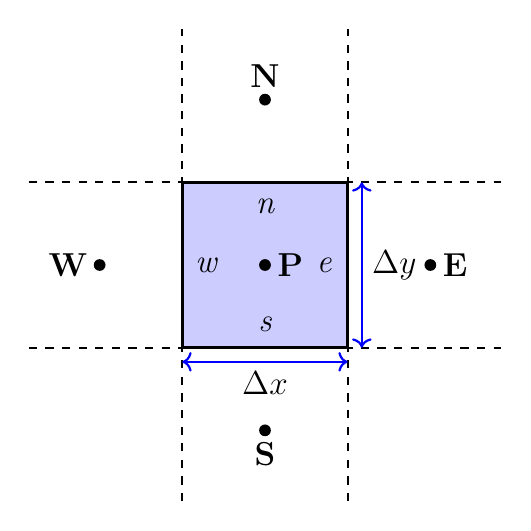
\begin{tikzpicture}[
        scale=0.6,
        font=\large,
        cv_node/.style={
            fill=black, 
            circle, 
            inner sep=1.5pt
        },
        node_label/.style={
            font=\large\bfseries,
            inner sep=2pt
        },
        face_label/.style={
            font=\large\itshape,
            inner sep=1pt
        }
    ]
        \def\nodedist{3.5cm}
        \def\grid_extent{5cm}
        
        \draw[dashed, line width=0.8pt] (-\grid_extent, \nodedist/2) -- (\grid_extent, \nodedist/2);
        \draw[dashed, line width=0.8pt] (-\grid_extent, -\nodedist/2) -- (\grid_extent, -\nodedist/2);
        \draw[dashed, line width=0.8pt] (\nodedist/2, -\grid_extent) -- (\nodedist/2, \grid_extent);
        \draw[dashed, line width=0.8pt] (-\nodedist/2, -\grid_extent) -- (-\nodedist/2, \grid_extent);

        \draw[line width=1.0pt, fill=blue!20] 
            (-\nodedist/2, -\nodedist/2) rectangle (\nodedist/2, \nodedist/2);
        
        \node[cv_node, label={[node_label]right:P}] (P) at (0,0) {};
        \node[cv_node, label={[node_label]above:N}] (N) at (0, \nodedist) {};
        \node[cv_node, label={[node_label]below:S}] (S) at (0, -\nodedist) {};
        \node[cv_node, label={[node_label]right:E}] (E) at (\nodedist, 0) {};
        \node[cv_node, label={[node_label]left:W}] (W) at (-\nodedist, 0) {};
        
        \node[face_label] at (\nodedist/2 - 0.5cm, 0) {e};
        \node[face_label] at (-\nodedist/2 + 0.5cm, 0) {w};
        \node[face_label] at (0, \nodedist/2 - 0.5cm) {n};
        \node[face_label] at (0, -\nodedist/2 + 0.5cm) {s};

        \draw[<->, thick, blue] 
            (\nodedist/2 + 0.3cm, -\nodedist/2) -- (\nodedist/2 + 0.3cm, \nodedist/2) 
            node[midway, right, text=black] {$\Delta y$};
        
        \draw[<->, thick, blue] 
            (-\nodedist/2, -\nodedist/2 - 0.3cm) -- (\nodedist/2, -\nodedist/2 - 0.3cm) 
            node[midway, below, text=black] {$\Delta x$};
            
    \end{tikzpicture}
    
    \caption{The 2D FVM grid notation.}
    \label{fvm_grid_exact}
\end{figure}

\bigskip

\textbf{3. Discretization at faces.}
We approximate the surface integrals from the previous point using the values at the faces' centers
\[
(F_n T_n - F_s T_s) + (F_e T_e - F_w T_w)
=(J^{\text{diff}}_n - J^{\text{diff}}_s) + (J^{\text{diff}}_e - J^{\text{diff}}_w),
\]
where $F_e=(\rho\,u_x)|_e\,\Delta y$ and $J_e^\text{diff}=(\Gamma\,\partial_xT)|_e\,\Delta y$ are the convective and diffusive fluxes through the eastern face and the others are defined similarly. Now we interpolate face values from nodal values. For the diffusive fluxes, we apply central differencing
\begin{alignat*}{2}
&J^{\text{diff}}_e = \Gamma\,\frac{T_E-T_P}{\Delta x}\,\Delta y
= D_e\,(T_E-T_P), \qquad &&D_e=\Gamma\frac{\Delta y}{\Delta x},\\
&J^{\text{diff}}_w = \Gamma\,\frac{T_P-T_W}{\Delta x}\,\Delta y
= D_w\,(T_P-T_W), \qquad &&D_w=\Gamma\frac{\Delta y}{\Delta x},\\
&J^{\text{diff}}_n = \Gamma\,\frac{T_N-T_P}{\Delta y}\,\Delta x
= D_n\,(T_N-T_P), \qquad &&D_n=\Gamma\frac{\Delta x}{\Delta y},\\
&J^{\text{diff}}_s = \Gamma\,\frac{T_P-T_S}{\Delta y}\,\Delta x
= D_s\,(T_P-T_S), \qquad &&D_s=\Gamma\frac{\Delta x}{\Delta y}
\end{alignat*}

And for the convective fluxes, with upwind differencing
\begin{align*}
T_e=
\begin{cases}
T_P,&F_e>0,\\
T_E,&F_e<0
\end{cases}
\qquad
T_w=
\begin{cases}
T_W,&F_w>0,\\
T_P,&F_w<0
\end{cases}
\end{align*}
Since $u_y = 0$, $F_n = F_s = 0$.

\bigskip

\textbf{4. Algebraic equation in an inner CV.}
The discretized flux balance reads
\[
a_P\,T_P=a_E\,T_E+a_W\,T_W+a_N\,T_N+a_S\,T_S+b_P
\]
where
\begin{alignat*}{2}
&a_E = D_e + \max(-F_e,0), \qquad &&a_W = D_w + \max(F_w,0),\\
&a_N = D_n, \qquad &&a_S = D_s,\\
&a_P = a_E+a_W+a_N+a_S+(F_e-F_w), \qquad &&b_{i,j} =0
\end{alignat*}

Once again, $u_y = 0 \implies F_n = F_s = 0$ and, by the continuity equation in the incompressible case, $F_e = F_w$ so $a_P$ has one less term. Physically, each term is a flux times temperature, in fact, using the fundamental measures $[\mathrm{M}]=\text{mass},\;[\mathrm{L}]=\text{length},\;[\mathrm{T}]=\text{time},\;[\mathrm{K}]=\text{temperature}$, we have
\begin{align*}
&[k]=\frac{\mathrm{W}}{\mathrm{m\,K}}=\frac{\mathrm{kg}\,\mathrm{m}}{\mathrm{s}^3\,\mathrm{K}} = \frac{[\mathrm{M}][\mathrm{L}]}{[\mathrm{T}]^3[\mathrm{K}]}\\
&[c_p]=\frac{\mathrm{J}}{\mathrm{kg\,K}}=\frac{\mathrm{m}^2}{\mathrm{s}^2\,\mathrm{K}} = \frac{[\mathrm{L}]^2}{[\mathrm{T}]^2[\mathrm{K}]}\\
&[\Gamma]=\frac{[k]}{[c_p]}=
\frac{\dfrac{[\mathrm{M}][\mathrm{L}]}{[\mathrm{T}]^3[\mathrm{K}]}}
{\dfrac{[\mathrm{L}]^2}{[\mathrm{T}]^2[\mathrm{K}]}}
= \frac{[\mathrm{M}]}{[\mathrm{L}][\mathrm{T}]} \;=\; [M][L]^{-1}[T]^{-1}\\
&[D_e]=[\Gamma]\frac{[\Delta y]}{[\Delta x]}
=[M][L]^{-1}[T]^{-1}\frac{[L]}{[L]}
=[M][L]^{-1}[T]^{-1}\\
&[F_e]=[\rho][u][\Delta y]
=[M][L]^{-3} \cdot [L][T]^{-1}[L]
=[M][L]^{-1}[T]^{-1}
\end{align*}
therefore
\[
[a_E] =[D_e + \max(-F_e,0)] = [M][L]^{-1}[T]^{-1}
\]
By similar computations for the other coefficients, we conclude that
\[
[a_P\,T_P]=[a_E\,T_E]=[a_W\,T_W]=[a_N\,T_N]=[a_S\,T_S]=[M][L]^{-1}[T]^{-1}[K],
\]
The unit of $b$ is not computed since it is everywhere equal to 0.

\bigskip

\textbf{5. CV indexing and boundaries.}
Consider the mesh described in Figure \ref{fvm_grid_exact}, we assign indices to the control volumes in the following manner
\begin{align*}
&i=1,\dots,n_y \quad\text{(spanwise direction, from upper to lower wall)},\\
&j=1,\dots,n_x \quad\text{(streamwise direction, from inlet to outlet)}
\end{align*}

The boundaries are
\[
\begin{cases}
\text{Inlet: } (i,j) = (i,1), & i\in\{1,\dots,n_y\},\\
\text{Outlet: } (i,j) = (i,n_x), & i\in\{1,\dots,n_y\},\\
\text{Lower wall: } (i,j) = (n_y, j), & j\in\{1,\dots,n_x\},\\
\text{Upper wall: } (i,j) = (1, j), & j\in\{1,\dots,n_x\}
\end{cases}
\]

An inner CV indexed by $(i,j)$ has neighbors:
\[
\begin{aligned}
W &\equiv (i,j-1) \quad &\text{(west neighbor)},\\
E &\equiv (i,j+1) \quad &\text{(east neighbor)},\\
S &\equiv (i+1,j) \quad &\text{(south neighbor)},\\
N &\equiv (i-1,j) \quad &\text{(north neighbor)}.
\end{aligned}
\]
With this convention \(W\) and \(E\) are located along the streamwise ($x$) direction, \(S\) and \(N\) are along the spanwise ($y$) direction, and the origin \((x,y)=(0,0)\) corresponds to the center of the top–left CV at the intersection between channel inlet and upper wall. The convention is outlined in Figure \ref{indexing_sketch_split}.
\begin{figure}[h!]
    \centering % Center the figure
    
    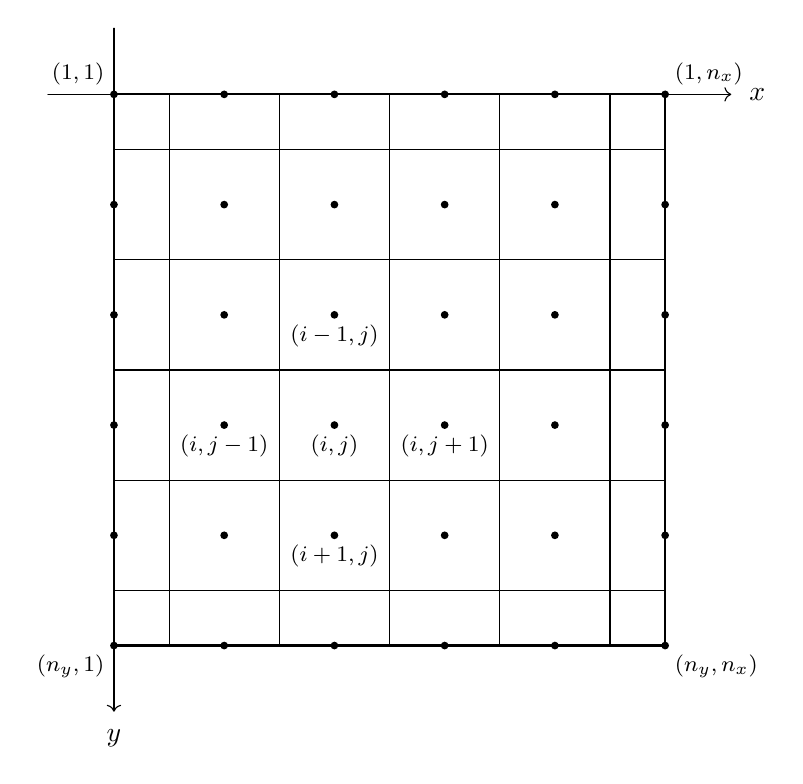
\begin{tikzpicture}[scale=1.4, line cap=round, line join=round]
        % parameters
        \def\nx{6}   % number of centers along x   (i = 1..nx)
        \def\ny{6}   % number of centers along y   (j = 1..ny)
        \def\dx{1} % interior-cell edge in x     (distance between centers)
        \def\dy{1} % interior-cell edge in y

        % domain frame: centers (1,1) at (0,0), (nx,ny) at ((nx-1)dx,(ny-1)dy)
        \pgfmathsetmacro{\xmin}{0}
        \pgfmathsetmacro{\ymin}{0}
        \pgfmathsetmacro{\xmax}{(\nx-1)*\dx}
        \pgfmathsetmacro{\ymax}{(\ny-1)*\dy}

        % external rectangle
        \draw[thick] (\xmin,\ymin) rectangle (\xmax,\ymax);

        % internal faces are mid-planes between adjacent centers
        % vertical faces
        \foreach \k in {1,...,\numexpr\nx-1\relax}{
            \pgfmathsetmacro{\x}{(\k-0.5)*\dx}
            \draw (\x,\ymin) -- (\x,\ymax);
        }
        
        % horizontal faces
        \foreach \l in {1,...,\numexpr\ny-1\relax}{
            \pgfmathsetmacro{\y}{(\l-0.5)*\dy}
            \draw (\xmin,\y) -- (\xmax,\y);
        }

        % centers: first layer lies on the frame, corners included
        \foreach \i in {1,...,\nx}{
            \foreach \j in {1,...,\ny}{
                \pgfmathsetmacro{\xc}{(\i-1)*\dx}
                \pgfmathsetmacro{\yc}{(\j-1)*\dy}
                \fill (\xc,\yc) circle (1-2pt);
            }
        }

        % axes
        \draw[->] (\xmin-0.6,\ymax) -- (\xmax+0.6,\ymax) node[right=3pt] {$x$};
        \draw[->] (0,\ymax+0.6) -- (0,\ymin-0.6) node[below=3pt] {$y$};

        % key labels
        \node[below left]   at (\xmin,\ymin) {\footnotesize $(n_y,1)$};
        \node[below right]  at (\xmax,\ymin) {\footnotesize $(n_y,n_x)$};
        \node[above left]   at (\xmin,\ymax) {\footnotesize $(1,1)$};
        \node[above right]  at (\xmax,\ymax) {\footnotesize $(1,n_x)$};

        % example generic (i,j)
        \pgfmathsetmacro{\xg}{(\nx>3 ? 2*\dx : \dx)}
        \pgfmathsetmacro{\yg}{(\ny>3 ? 2*\dy : \dy)}
        \node[below] at (\xg,\yg) {\footnotesize $(i,j)$};

        \pgfmathsetmacro{\xg}{(\nx>3 ? \dx : \dx)}
        \node[below] at (\xg,\yg) {\footnotesize $(i,j-1)$};

        \pgfmathsetmacro{\xg}{(\nx>3 ? 3*\dx : \dx)}
        \node[below] at (\xg,\yg) {\footnotesize $(i,j+1)$};

        \pgfmathsetmacro{\xg}{(\nx>3 ? 2*\dx : \dx)}
        \pgfmathsetmacro{\yg}{(\ny>3 ? \dy : \dy)}
        \node[below] at (\xg,\yg) {\footnotesize $(i+1,j)$};

        \pgfmathsetmacro{\yg}{(\ny>3 ? 3*\dy : \dy)}
        \node[below] at (\xg,\yg) {\footnotesize $(i-1,j)$};
    \end{tikzpicture}
    
    \caption{Indexing convention.}
    \label{indexing_sketch_split}
\end{figure}

\bigskip

\textbf{6. DOF numbering and mapping.}
Once discretized, the unknown $T$ is a vector of $N = n_x \cdot n_y$ values. We number these $N$ degrees of freedom (DOFs) by flattening $(i,j)$ into a single index $n$ with row-major, top-to-bottom ordering
\[
n = (i-1)\,n_x + j=1,\dots,n_x n_y
\]
For a generic inner CV of DOF index $n$, its neighbors are
\[
E:n+1,\quad W:n-1,\quad N:n-n_x,\quad S:n+n_x
\]
While the boundary DOFs are
\begin{alignat*}{2}
&\text{Inlet: } n = (i-1)n_x + 1, \qquad&& i \in \{1,\dots,n_y\}, \\
&\text{Outlet: } n = (i-1)n_x + n_x, \qquad&& i \in \{1,\dots,n_y\}, \\
&\text{Lower wall: } n = (n_y-1)n_x + j, \qquad&& j \in \{1,\dots,n_x\}, \\
&\text{Upper wall: } n = j, \qquad&&j \in \{1,\dots,n_x\}
\end{alignat*}

\bigskip

\textbf{7. Assembly of the matrix A and Inlet Boundary.}
With our convention, the equation of the the n-th control volume $a_P\,T_P=a_W\,T_W+a_E\,T_E+a_S\,T_S+a_N\,T_N+b_P$ becomes
$$a_{n,n-n_x}\,T_{n-n_x} + a_{n,n-1}\,T_{n-1}+a_{n,n}\,T_{n}+a_{n,n+1}\,T_{n+1}+a_{n,n+n_x}\,T_{n+n_x}=b_n$$
This linear system of equations is described by a matrix $A\in \mathbb{R}^{N\times N}$ and a vector $b\in \mathbb{R}^N$ whose entries, for inner CVs, are
\begin{align*}
&A(n, n) = a_P, \quad A(n, n+1) = -a_E, \quad A(n, n-1) = -a_W, \\
&A(n, n+n_x) = -a_N, \quad A(n, n-n_x) = -a_S, \quad b(n) = 0
\end{align*}
At the inlet boundary (\(1 \leq i \leq n_y\), \(j=1\)), \(T = T_{\text{in}}\), thus
\[
A(n, :) = 0, \quad A(n, n) = 1, \quad b(n) = T_{\text{in}}, \quad \text{where } n = (i-1)n_x + 1
\]

\bigskip

\textbf{8. Outlet Boundary.}
For outlet CVs (\(1 \leq i \leq n_y\), \(j = n_x\)), the Neumann condition \(\partial T/\partial x = 0\) leads to $a_E = 0$. Numerically
\begin{align*}
&A(n, n) = a_P, \quad A(n, n+1) = 0, \quad A(n, n-1) = -a_W, \quad A(n, n+n_x) = -a_N, \\
&A(n, n-n_x) = -a_S, \quad b(n) = 0, \quad \text{where } n = (i-1)n_x + n_x
\end{align*}

\bigskip

\textbf{9. Wall Boundaries.}
For lower wall (\(i=n_y\), \(1 \leq j \leq n_x\)) and upper wall (\(i = 1\), \(1 \leq j \leq n_x\)) CVs, \(T = T_{\text{wall}}\), so
\[
A(n, :) = 0, \quad A(n, n) = 1, \quad b(n) = T_{\text{wall}}, \quad \text{where } n = j \lor n=(n_y-1)n_x + j
\]
Note that corner CVs (e.g., \((i=1,j=1)\)) are assigned to walls to avoid boundary condition conflicts.

\bigskip

\textbf{10. Physical Parameter Calculation.}
Consider the following values for the fluid's physical properties: $\rho = 1\ \text{kg/m}^3$, $c_p = 10\ \text{J/(K $\cdot$ kg)}$, $k = 0.12\ \text{W/(m $\cdot$ K)}$, $\nu = 10^{-2}\ \text{m}^2/\text{s}$. Assume also that $L = 10\ \text{m}$, $H = 1\ \text{m}$, and that $\mathrm{Pe} = \rho \cdot u_\text{mean} \cdot (2H) / \Gamma = 16.5$. Then
\begin{align*}
    &\Gamma = \frac{k}{c_p} = \frac{0.12}{10} = 0.012\ \frac{\text{kg}}{m \cdot \text{s}}, \\
    &u_{\text{mean}} = \frac{Pe \cdot \Gamma}{2H \cdot \rho} = \frac{16.5 \cdot 0.012}{2 \cdot 1 \cdot 1} = 0.099\ \text{m/s}, \\
    &\mathrm{Re} = \frac{2H u_{\text{mean}}}{\nu} = \frac{2 \cdot 1 \cdot 0.099}{10^{-2}} = 19.8
\end{align*}

Since Re is much lower than the threshold value of 2300, so the flow is expected to be laminar.

\bigskip

\textbf{11. Coarse Mesh Solution and Visualization.}
Assume $T_\text{inlet} = 50^\circ C$ and $T_\text{wall} = 100^\circ C$. On a coarse mesh with \(n_x = 50\), \(n_y = 5\), the temperature field results physically reasonable, as shown in Figure \ref{temperature_field}.

\begin{figure}[H]
    \centering
    \includegraphics[width=1\textwidth]{Latex/MATLABfigures/11.png} 
    \caption{Channel temperature field (\(n_x=50\), \(n_y=5\)).}
    \label{temperature_field}
\end{figure}

\bigskip

\textbf{12. Boundary conditions verification.}
As demonstrated by the plots in Figure \ref{boundary_condition}, the solution respects all boundary conditions. Indeed we can see that: for the inlet the solution assumes the value $T_\text{wall} = 100^\circ C$ at the edges and the value $T_\text{inlet} = 50^\circ C$ for the internal nodes; at the outlet the functions $T(x,0.75)$ and $T(x,0.5)$ becomes flat when they reach $L=10\,m$, this means that their derivative with respect to x, at the end of the channel, is zero, as stated by the Neumann conditions; for the two horizontal walls is clear that the value remain constant to $T_\text{wall} = 100^\circ C$ both at $y=0$ and $y=H$.

\begin{figure}[H]
    \centering
    \includegraphics[width=0.9\textwidth]{Latex/MATLABfigures/12.png} 
    \caption{Top left plot shows how our solution assumes the inlet boundary condition; bottom left and bottom right respectively show how our solution correctly assumes the boundary conditions for the lower and upper wall; top right plot shows streamwise temperature evolution of our solution evaluated at two different heights (y=0.75, y=0.5), indeed we observe a Neumann condition at x=L.}
    \label{boundary_condition}
\end{figure}

\bigskip

\textbf{13. Temperature plots.} 
The 2D plot of the solution $T(x,y)$ can be seen in Figure \ref{temperature_field}. The outlet temperature is shown in Figure \ref{outlet_temperature}, while in Figure \ref{cent_mean_temp} the centerline temperature and the weighted mean temperature are plotted together with the entry length ($x_e = 2.449$). Note that the weighted mean temperature, defined as follows, is computed numerically, summing up all the contributions over the spanwise direction, in order to approximate the two integrals.

\begin{align}
    T_{mean}(x) = \dfrac{\int_{0}^{H}u_x(y)T(x,y)dy}{\int_{0}^{H}u_x(y)dy}
    \label{T_mean_formula}
\end{align}

\begin{figure}[H]
    \centering
    \includegraphics[width=0.6\textwidth]{Latex/MATLABfigures/13_1.png} 
    \caption{Temperature field at the outlet.}
    \label{outlet_temperature}
\end{figure}

\begin{figure}[H]
    \centering
    \includegraphics[width=0.6\textwidth]{Latex/MATLABfigures/13_2.png} 
    \caption{Centerline and velocity-weighted mean temperature.}
    \label{cent_mean_temp}
\end{figure}

\bigskip

\textbf{14. Iterative methods.} 
In order to solve the system $AT=b$, instead of the Matlab backslash, we implement the Successive Over Relaxation method: starting from a suitable initial guess $T^0$, that respect the boundary conditions (for example a $T^0$ equal to $50^\circ C$ on the inlet and $100^\circ C$ on the two walls), the method monitors the values of relative iteration error $||T^k - T^{k-1}||_2\,/\,||T^{k-1}||_2 $ (Figure \ref{relative_error}), and the normalized residuals $||AT^k - b||_2\,/\,||diag(A)\,T^k||_2 $ (Figure \ref{residuals}), and stop when both are smaller than the tolerance $10^{-5}$. The SOR method is an algorithm that includes a relaxation parameter, $w$, to control its convergence. The choice of this parameter is critical: setting $w=1$ simplifies the algorithm to the standard Gauss-Seidel method. In contrast, setting w in the range $1<w<2$ (in this case, $w=1.5$) applies over-relaxation, a technique designed to accelerate convergence. The simulation using the Gauss-Seidel method took 35 iterations to meet the stopping criteria, while the over-relaxation method converged significantly faster, requiring only 23 iterations.

\begin{figure}[H]
    \centering
    \includegraphics[width=0.7\textwidth]{Latex/MATLABfigures/14_1.png} 
    \caption{Temperature field at the outlet.}
    \label{relative_error}
\end{figure}

\begin{figure}[H]
    \centering
    \includegraphics[width=0.7\textwidth]{Latex/MATLABfigures/14_2.png} 
    \caption{Centerline and velocity-weighted mean temperature.}
    \label{residuals}
\end{figure}

\bigskip

\textbf{15. Nusselt Number computation}
Consider the Nusselt Number defined as 
\begin{align}
    \mathrm{Nu} = \frac{\partial T / \partial n}{\Delta T / (2H)}
    \label{nusselt_formula}
\end{align}
where $\Delta T = T_{wall}\,-T_{mean}$ is the difference between the wall temperature and the velocity-averaged mean temperature $T_{mean}$ defined earlier. For laminar flows in plane channels, as shown by \cite{nusselt}, $\mathrm{Nu}(x)$ decreases in the entrance region, but far enough downstream of the inlet it approaches a constant value independent of the Péclet number. To remark that we're working in the case of uniform wall temperature, the Nusselt number is indicated as $\mathrm{Nu_T}(x)$. Numerically, we compute $\mathrm{Nu_T}(x)$ by approximating the velocity-averaged mean temperature (as in question 13) and the normal derivative of the temperature at the wall using a finite difference, the resulting $\mathrm{Nu_T}(x)$ along the lower wall can be observed in Figure \ref{nusselt}. It tends to a limit of 6.68, which we found to be reasonably close to the expected value of 7.54. 
However, contrary to theoretical expectations, the trend also presents a sudden spike in Nusselt value near the outlet. This feature is a numerical artifact, not a physical phenomenon, and is caused by a conflict between the physics of the flow and the Neumann boundary condition. Indeed, a Neumann null outlet condition means that the temperature profile is no longer changing in the direction of the flow. Apparently, this is pacific since it's also what we expect from the definition of \textit{fully developed} flow. In reality, there is still heat transfer occurring at the outlet, so such condition on the gradient is too restrictive, leading to a model incapable of capturing the essence of our phenomenon. 
Numerically, what happens is that the solver has to forcibly bend the temperature profile in the last few cells of the mesh to satisfy the Neumann condition. This distortion then pollutes the entire temperature field upstream of the outlet, rendering the calculated wall gradient smaller than what is expected form experiments, and leading to the artificial spike in the value of $\mathrm{Nu}$ we observe.

\begin{figure}[H]
    \centering
    \includegraphics[width=0.7\textwidth]{Latex/MATLABfigures/15.png} 
    \caption{Nusselt Number along the lower wall.}
    \label{nusselt}
\end{figure}

\bigskip

\textbf{16. Mesh refinement study.} 
To ensure that the numerical solution is independent of the grid resolution, a mesh convergence study was performed. The simulation was run on four progressively refined meshes, as shown in Table \ref{mesh_refinement}. To evaluate the convergence between these cases, several key quantities of interest were computed and compared. These include the  the entry length $x_e$, Table \ref{mesh_refinement}, the outlet temperature profile $T_o(y)$, Figure \ref{outlet_temperature_profile}, the centerline temperature $T_c(x)$, Figure \ref{centerline_temperature}, the velocity averaged mean temperature $T_{mean}(x)$ defined by \ref{T_mean_formula}, Figure \ref{mean_temperature_profile} and the local Nusselt number $Nu(x)$, defined by \ref{nusselt_formula}, along the heated wall, Figure \ref{nusselt_profile}. The results can be seen in the plots below:

\begin{table}[H]
    \centering
        \begin{tabular}{|c|c|c|} 
        \hline
        $\mathbf{n_x}$ & $\mathbf{n_y}$ & \textbf{Entry Length} \\ 
        \hline
        50 & 5 & 2.449 \\ 
        \hline
        100 & 11 & 2.3232 \\ 
        \hline
        200 & 21 & 2.2111 \\ 
        \hline
        400 & 41 & 2.1805 \\
        \hline
        \end{tabular}
    \caption{The Mesh refinement and the corresponding entry length values.}
    \label{mesh_refinement}
\end{table}

\begin{itemize}
    
    \item This plot of the outlet temperature profile demonstrates successful grid convergence. The coarsest mesh, "Refinement level 1", is under-resolved and shows non-physical profile with a minimum temperature (around 99.965$^\circ$C) that is lower than the other cases. As the mesh is refined to "Refinement level 2" and "Refinement level 3", the solution curves become progressively smoother and shift upwards, indicating that they are approaching a stable solution.
    
    \begin{figure}[H]
        \centering
        \includegraphics[width=0.6\textwidth]{Latex/MATLABfigures/16_1.png} 
        \caption{Temperature at the outlet.}
        \label{outlet_temperature_profile}
    \end{figure}

    \item This plot of the centerline temperature profile also shows clear evidence of grid convergence. A noticeable, though small, gap exists between "Refinement level 1" and "Refinement level 2", particularly in the thermal entrance region. The most important finding is that the curves for Level 3 and Level 4 are visually identical across the entire domain. This indicates the solution has fully stabilized, and further mesh refinement does not alter the result.
    
    \begin{figure}[H]
        \centering
        \includegraphics[width=0.8\textwidth]{Latex/MATLABfigures/16_2.png} 
        \caption{Centerline temperature profile.}
        \label{centerline_temperature}
    \end{figure}

    \item The plot for the velocity-averaged mean temperature provides further strong confirmation of grid convergence. "Refinement level 1" is slightly under-resolved, predicting a slower temperature rise in the entrance region compared to the finer grids. The solution progressively improves with "Refinement level 2", which is closer to the final solution. Also in this plot can be appreciated an excellent agreement between "Refinement level 3" and "Refinement level 4". These two curves are visually indistinguishable over the entire length of the domain, demonstrating that the solution has fully stabilized.
    
    \begin{figure}[H]
        \centering
        \includegraphics[width=0.8\textwidth]{Latex/MATLABfigures/16_3.png} 
        \caption{Velocity averaged mean temperature profile.}
        \label{mean_temperature_profile}
    \end{figure}

    \item The plot of the local Nusselt number provides excellent evidence of grid convergence. "Refinement level 1" is significantly under-resolved, predicting a fully developed Nu value of only 6.7, which is far from the theoretical prediction. As the mesh is refined, the solution curves for Level 2, Level 3, and Level 4 clearly and asymptotically converge towards the theoretical value of 7.54, predicted in \cite{nusselt}. The zoomed-in view shows that the change between Level 3 and Level 4 is very small, confirming the solution has stabilized. It is also worth noting that the small up-tick in Nu near the outlet) is present at all refinement levels. This indicates it is not a grid resolution error but rather a numerical artifact, stemming from the influence of the outlet boundary condition.
    
    \begin{figure}[H]
        \centering
        \includegraphics[width=0.8\textwidth]{Latex/MATLABfigures/16_4.png} 
        \caption{The Nusselt number profile.}
        \label{nusselt_profile}
    \end{figure}
\end{itemize}

\bigskip

\textbf{17. QUICK discretization.} To evaluate the impact of the numerical discretization scheme on the solution accuracy, the simulation is re-run using the QUICK scheme for the convective term, replacing the First-Order Upwind scheme used previously. QUICK is a higher-order scheme designed to reduce the numerical diffusion inherent in first-order methods like UD. After the discretization with QUICK the algebraic equation is as follows:

\[
a_P\,T_P=a_E\,T_E+a_W\,T_W+a_N\,T_N+a_S\,T_S+b_P
\]
where
\begin{alignat*}{2}
&a_{WW}=-\max(0,\frac{F_e}{8}) \qquad &&a_{EE}=-\max(0,-\frac{F_e}{8}),\\
&a_E = D_e -\max(0,\frac{3F_e}{8})+\max(0,\frac{-6F_e}{8})-\max(0,-\frac{F_w}{8}), \qquad &&a_N = D_n,\\
&a_W = D_w +\max(0,\frac{6F_w}{8})+\max(0,\frac{F_e}{8})-\max(0,-\frac{3F_w}{8}), \qquad &&a_S = D_s,\\
&a_P = a_E+a_W+a_N+a_S, \qquad &&b_{i,j} =0
\end{alignat*}

The solution is computed on the same four progressively refined meshes to compare the convergence behavior of both schemes. The entrance length $x_e$ is used as the primary metric for this comparison, as shown in the Tables below.

\begin{table}[H]
    \centering
    \begin{minipage}{.45\textwidth}
        \centering
        \begin{tabular}{|c|c|c|} 
            \hline
            $\mathbf{n_x}$ & $\mathbf{n_y}$ & \textbf{Entry Length (UD)} \\ 
            \hline
            50 & 5 & 2.449 \\ 
            \hline
            100 & 11 & 2.3232 \\ 
            \hline
            200 & 21 & 2.2111 \\ 
            \hline
            400 & 41 & 2.1805 \\
            \hline
        \end{tabular}
    \caption{The entry length computed with the UD method.}
    \label{entry_lenght_table_ud}
    \end{minipage}
    \hspace{0.05\textwidth}
    \begin{minipage}{.45\textwidth}
        \centering
        \begin{tabular}{|c|c|c|} 
            \hline
            $\mathbf{n_x}$ & $\mathbf{n_y}$ & \textbf{Entry Length (QUICK)} \\ 
            \hline
            50 & 5 & 2.449 \\ 
            \hline
            100 & 11 & 2.2222 \\ 
            \hline
            200 & 21 & 2.1608 \\ 
            \hline
            400 & 41 & 2.1554 \\
            \hline
        \end{tabular}
    \caption{The entry length computed with the QUICK method.}
    \label{entry_lenght_table_quick}
    \end{minipage}
\end{table}

The plot in Figure \ref{entry_length_comparison} shows the computed $x_e$ for both schemes, and illustrates the superior convergence rate of QUICK. Both methods start with a similarly inaccurate entry length of 2.45 on the coarsest mesh (black dot). However, the "Upwind" scheme's solution converges very slowly and gradually, with significant gaps remaining even between the finest meshes (blue and red dots), indicating it has not yet reached a grid-independent solution. In contrast, the "Quick" scheme converges much more rapidly; after a large jump from Mesh 1 (black) to Mesh 2 (green), the values for Mesh 3 (blue) and Mesh 4 (red) are extremely close to each other. 

\begin{figure}[H]
    \centering
    \includegraphics[width=0.6\textwidth]{Latex/MATLABfigures/17_1.png} 
    \caption{The entry length comparison between UD and QUICK, as shown in the Tables \ref{entry_lenght_table_ud}, \ref{entry_lenght_table_quick}.}
    \label{entry_length_comparison}
\end{figure}

The plot in Figure \ref{relative_entry_length_comparison}, which displays the relative error with respect to the finest mesh solution (red dot), provides a quantitative confirmation of QUICK's higher-order accuracy. The "Upwind" scheme's error decreases slowly, starting high at 12.5\% (black dot), reducing to 6.5\% (green dot), and remaining over 1\% even on Mesh 3 (blue dot). In contrast, the "Quick" scheme's error drops dramatically: while starting at a similar 13.5\%, its error on Mesh 2 (green dot)is already less than half that of the Upwind scheme, and it becomes nearly zero on Mesh 3 (blue dot). This rapid error reduction proves the superior convergence rate of the QUICK scheme.

\begin{figure}[H]
    \centering
    \includegraphics[width=0.6\textwidth]{Latex/MATLABfigures/17_2.png} 
    \caption{Relative variation for $x_e$ with respect to the finest mesh, for UD and QUICK.}
    \label{relative_entry_length_comparison}
\end{figure}

\bigskip

\textbf{18. Independent $n_x$ and $n_y$ refinement} 
Previous simulations used meshes with approximately square control volumes to perform a standard grid convergence study. While this approach is robust, it may not be the most computationally efficient. It is possible that the solution is more sensitive to resolution in one direction (e.g., the transverse $y$-direction, where gradients are steep) than the other (e.g., the axial $x$-direction). To test this, two separate series of simulations are conducted and the entrance length will be used as the key scalar metric for comparison.

\begin{enumerate}

    \item Fixed streamwise Resolution ($n_x=400$): The transverse resolution is varied using meshes of ($n_x, n_y$) = (400, 5), (400, 11), and (400, 21), showing the solution's sensitivity to $\Delta y$.

    \item Fixed spanwise Resolution ($n_y=41$): The axial resolution is varied using meshes of ($n_x, n_y$) = (100, 41), (200, 41), and (400, 41), showing the solution's sensitivity to $\Delta x$.

\end{enumerate}

The plot in Figure \ref{axial_refinement} compares the effect of streamwise and spanwise refinement on the minimum Nusselt number. The orange line is perfectly horizontal at a value of approximately $Nu \approx 7.57$, demonstrating that the solution is completely insensitive to the axial mesh resolution $\Delta x$ once the transverse resolution is sufficient (here $n_y=41$). In contrast, the blue line shows a very strong dependence on the transverse resolution. As $\Delta y$ is refined (moving left on the plot), the computed minimum $Nu$ value clearly converges upwards from a highly inaccurate $\approx 6.7$ and progressively approaches the theoretical value of 7.54. This analysis proves that the transverse resolution $\Delta y$ is the single most critical factor for accuracy, and that a high-aspect-ratio mesh (e.g., $n_x=100, n_y=41$) is more efficient than a 'square' mesh for this problem.

\begin{figure}[H]
    \centering
    \includegraphics[width=0.7\textwidth]{Latex/MATLABfigures/18.png} 
    \caption{Minimum Nusselt number for varying $n_x$ and $n_y$.}
    \label{axial_refinement}
\end{figure} 

\textbf{19. Changing the Péclet Number.}
The plots in Figures \ref{peclet_50} and \ref{peclet_100} show a qualitative comparison of the full two-dimensional temperature fields, $T(x,y)$, at two different Péclet numbers, $Pe$. The two plots clearly visualize the physical meaning of the Péclet number. The first plot (Figure \ref{peclet_50}), representing $Pe=50$, shows a case where physical diffusion is relatively strong: as a result, heat from the hot walls diffuses into the central core fluid much more rapidly, causing the blue and cold region to be shorter and wider, smearing the profile and causing it to dissipate by $x \approx 5$ m. In contrast, the second plot (Figure \ref{peclet_100}), representing $Pe=100$, shows a flow dominated by advection. The flow's stiffness resists the diffusive effects from the wall, advecting the cold inlet temperature much further downstream. This results in a  longer cold core. 

\begin{figure}[H]
    \centering
    \includegraphics[width=1\textwidth]{Latex/MATLABfigures/19_1.png} 
    \caption{Temperature field with $P_e=50$}
    \label{peclet_50}
\end{figure} 

\begin{figure}[H]
    \centering
    \includegraphics[width=1\textwidth]{Latex/MATLABfigures/19_2.png} 
    \caption{Temperature field with $P_e=100$}
    \label{peclet_100}
\end{figure} 

\bigskip

\textbf{20. Neumann boundary condition at the walls.}
We now want to impose a Neumann condition \(k \cdot \partial T/\partial x = q_\text{wall}\) on the lower (\(i=n_y\), \(1 \leq j \leq n_x\)) and upper (\(i = 1\), \(1 \leq j \leq n_x\)) wall CVs. This leads to:

\begin{itemize}

    \item Uppermost CVs (Non-Corner) (for $i=1, 1 < j < n_x$)
    \begin{align*}
    &a_N = 0 \\
    &a_P = a_E + a_W + a_S \\
    &b(n) = \frac{q_{wall}}{c_p} \Delta x
    \end{align*}
    
    \item Lowermost CVs (Non-Corner) (for $i=n_y, 1 < j < n_x$)
    \begin{align*}
    &a_N = 0 \\
    &a_P = a_E + a_W + a_N \\
    &b(n) = \frac{q_{wall}}{c_p} \Delta x
    \end{align*}

    \item Upper-Left Corner ($i=1, j=1$): This cell is an inlet, so the Dirichlet condition $T_P = T_{\text{in}}$ overrides the Neumann wall condition. The equation is simply $T_P = T_{\text{in}}$.
    
    \item Lower-Left Corner ($i=n_y, j=1$): This cell is also an inlet, and the Dirichlet condition $T_P = T_{\text{in}}$ overrides the Neumann wall condition. The equation is $T_P = T_{\text{in}}$.

    \item Upper-Right Corner ($i=1, j=n_x$): This cell combines the outlet and upper wall conditions.
    \begin{align*}
    &a_E = 0 \\
    &a_N = 0 \\
    &a_P = a_W + a_S \\
    &b(n) = \frac{q_{wall}}{c_p} \Delta x
    \end{align*}
    
    \item Lower-Right Corner ($i=n_y, j=n_x$): This cell combines the outlet and lower wall conditions.
    \begin{align*}
    &a_E = 0 \\
    &a_S = 0 \\
    &a_P = a_W + a_N \\
    &b(n) = \frac{q_{wall}}{c_p} \Delta x
    \end{align*}

\end{itemize}

The plot in Figure \ref{wall_neumann} shows that the temperature field for the constant heat flux ($q_{\text{wall}} = 10\,W/m^2$) case looks physically reasonable. The simulation correctly captures the uniform inlet temperature at $x=0$. As the fluid flows down the channel, heat is added from both the upper and lower walls, causing the entire fluid to heat up continuously.

\begin{figure}[H]
    \centering
    \includegraphics[width=1\textwidth]{Latex/MATLABfigures/20_1.png} 
    \caption{Temperature field with Neumann conditions at the wall.}
    \label{wall_neumann}
\end{figure} 

The plots in Figure \ref{boundary_wall_neumann} provide an a posteriori check that the boundary conditions have been correctly implemented. The Inlet plot confirms that the Dirichlet inlet condition is correctly enforced, showing a constant temperature across the entire $y$-direction at $x=0$. The two plots Wall (y = 0) and Wall (y = H) shows the computed wall temperatures, they correctly start at $50^\circ C$ at $x=0$, matching the inlet temperature, and then show a continuous, near-linear rise as the fluid is heated. This behavior is the correct physical consequence of a constant positive heat flux, $q_{wall} > 0$.  The outlet plot shows shows temperature evolution of the solution evaluated at the last two CVs, we observe a Neumann condition at x=L since the solution is not changing much in the x direction.

\begin{figure}[H]
    \centering
    \includegraphics[width=0.9\textwidth]{Latex/MATLABfigures/20_2.png} 
    \caption{Top left plot shows how our solution assumes the inlet boundary condition; bottom left and bottom right respectively show how our solution correctly assumes the boundary conditions for the lower and upper wall; top right plot shows temperature evolution of the solution evaluated at the last two CVs.}
    \label{boundary_wall_neumann}
\end{figure} 

The plot in Figure \ref{nusselt_wall_neumann} exhibits a very high Nusselt number near the inlet x=0 which then decays rapidly as the thermal boundary layer develops. Note that on the first cell $Nu = 0$, this is because the Dirichlet boundary condition are imposed also on the corners of the inlet, and this leads to a null denominator in Formula \ref{nusselt_formula}. Beyond the entrance section, the flow becomes thermally fully-developed, and the Nusselt number correctly settles at a constant value, which for this case is $Nu \approx 6.9$. The small, sudden drop in $Nu$ observed at the very end of the channel is a numerical artifact, and is caused by the approximate nature of the numerical boundary condition imposed at the finite domain outlet, which can slightly influence the solution just upstream of the boundary. Note that in this case $Nu$ experience a drop, while when constant wall condition were imposed $Nu$ slightly increase at the end of the domain, as shown in Figure \ref{nusselt}.

\begin{figure}[H]
    \centering
    \includegraphics[width=0.6\textwidth]{Latex/MATLABfigures/20_3.png} 
    \caption{$Nu_q(x)$ along the lower wall.}
    \label{nusselt_wall_neumann}
\end{figure} 

\bigskip

\textbf{21. Global conservation of thermal energy.}
After obtaining a converged solution, we check if the numerical model globally conserves thermal energy. This requires a systematic accounting of all heat fluxes crossing the boundaries of the computational domain. The net sum of these fluxes should ideally be zero, confirming that energy is neither created nor destroyed, in accordance with the First Law of Thermodynamics.

\begin{table}[H]
    \centering
        \begin{tabular}{|c|c|c|c|c|} 
        \hline
        & \textbf{Inlet} & \textbf{Outlet} & \textbf{Wall (y=0)} & \textbf{Wall (y=H)} \\ 
        \hline
        \textbf{Diffusive flux} & 0 & 0 & 0 & 0 \\ 
        \hline
        \textbf{Convective flux} &0 & 0 & 0 & 0 \\ 
        \hline
        \end{tabular}
    \caption{Values of the diffusive and convective thermal flux at the boundaries.}
    \label{boundary_thermal_conservation}
\end{table}

The global thermal energy balance, considering all the contributions, is $.$. This shows that in the simulation the total energy is conserved.

\bigskip

\textbf{22. Non uniform wall boundary conditions.}
que

\bibliographystyle{plain}
\bibliography{literature}

\end{document}
